\begin{figure*}[t]
  \title{Accuracy at Various Hidden Unit/Layer Combinations}
\centering

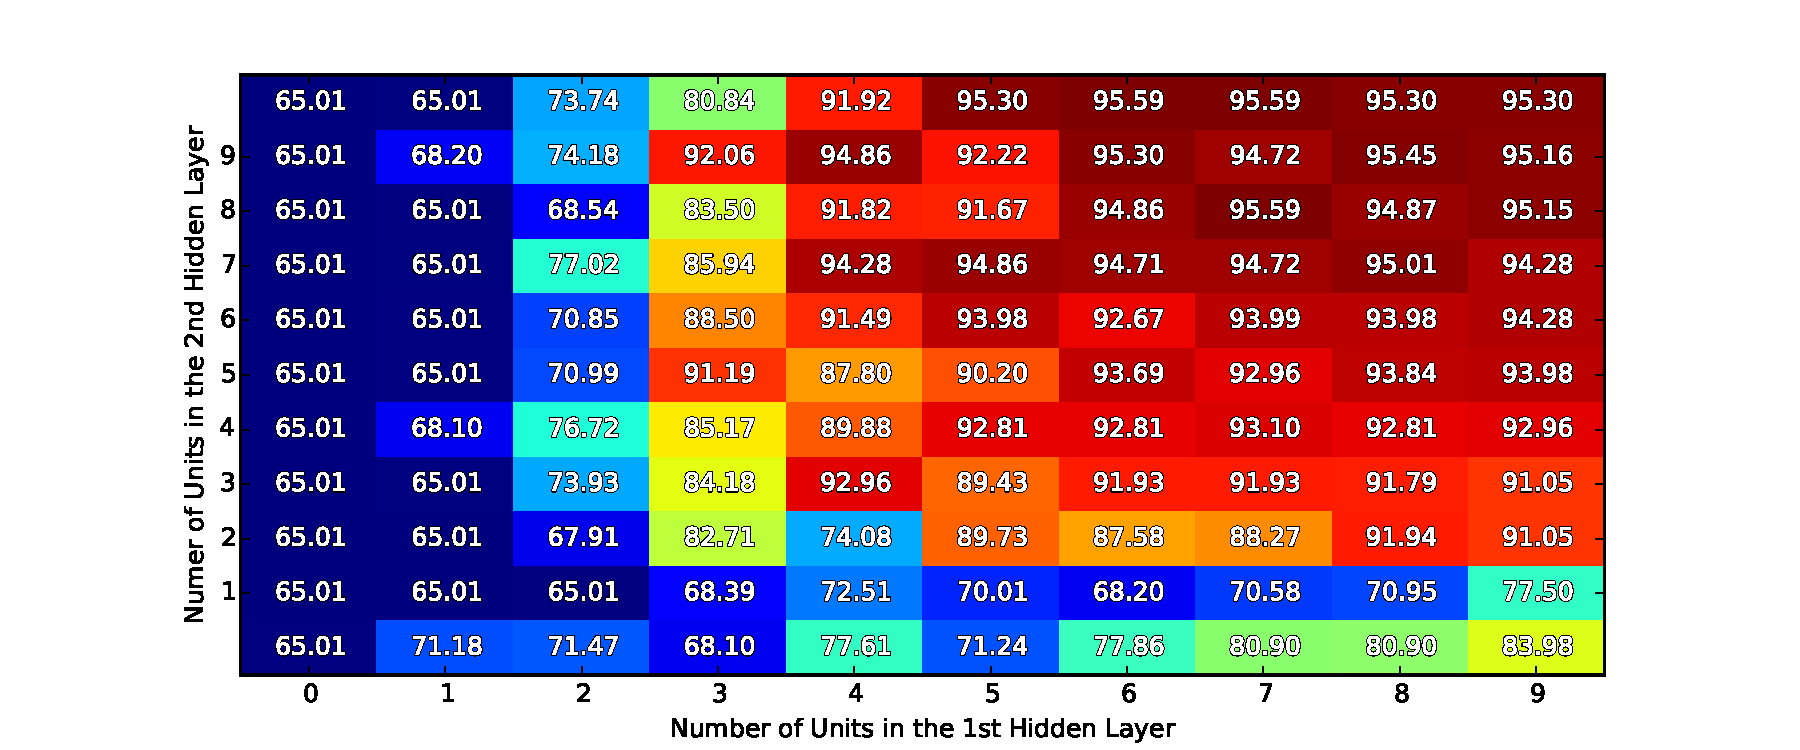
\includegraphics[width=\textwidth]{figs/wbcd_table}

\caption {Accuracy for neural networks with one and two hidden layers. Entry \((i,j)\) represents a neural network with \(j\) units in the \nth{1} hidden layer and \(i\) units in the \nth{2} hidden layer ({\em i.e.,} row 0 represents neural networks with only one hidden layer). All combinations were trained for 10 epochs and 10-fold cross validation.}
\label{fig:wbcd_table}
\end{figure*}

Figure~\ref{fig:wbcd_table} shows the results from our search through the parameter space of hidden unit combinations.
An entry \((i,j)\) in the table is the predictive accuracy of a neural network with \(j\) perceptrons in the \nth{1} hidden layer and \(i\) perceptrons in the \nth{2} hidden layer.
We overlay a heat map on the table to better quantify how the choices for \((i,j)\) combinations effects predictive accuracy.
For example, it is clear from the table a neural network with one hidden layer ({\em e.g.,} \(j=0\)) performs well (above 80\% predictive accuracy) if it consists of 9 or more perceptrons.
Additionally, for low values of \(j\) (less than 5), increasing the number of perceptrons in the \nth{2} hidden layer does not improve predictive accuracy substantially.
We posit this is because the representational power of the \nth{1} hidden layer is too low and the feature space is being compressed to heavily that no amount of additional complexity at the \nth{2} hidden layer can compensate.

Although we do not see this is Figure~\ref{fig:wbcd_table}, ideally we want to see a concentrated area of red surrounded by blue.
We speculate this did not occur because the target concept for the WBC data set was very easy to learn and therefore, adding more perceptrons at each hidden layer does not lead to significant overfitting of the data.
Normally, it is advantageous to pick an \((i,j)\) combination that falls on the horizon.
However, we chose to proceed with the best \((i,j)\) combination from the table.
Note, for the space we searched this is \((13,14)\).

\begin{figure}[t]
\centering

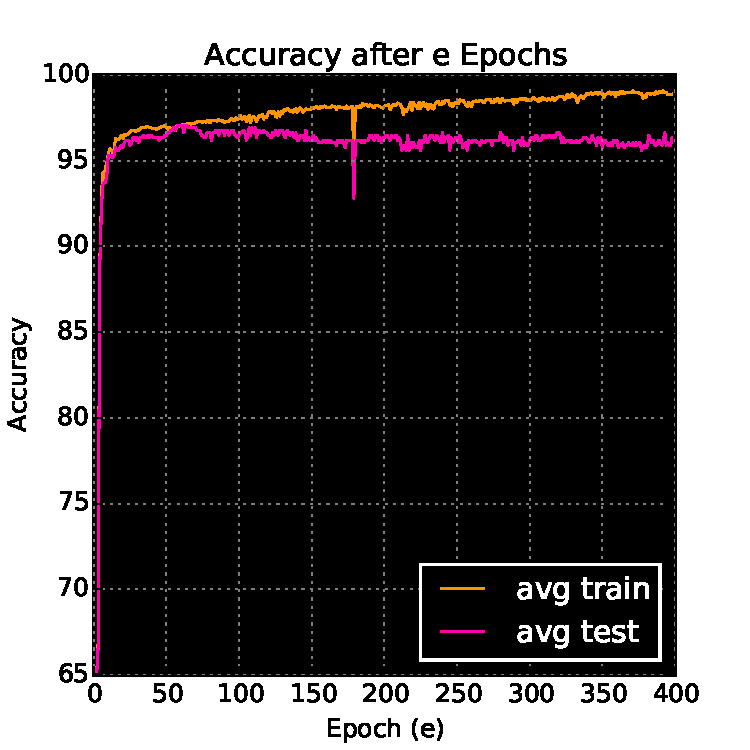
\includegraphics[width=0.95\columnwidth]{figs/wbcd_iterative}

\caption {Average accuracy on the training and test sets at every epoch from 1 to 400 for a neural network with 14 units at the \nth{1} hidden layer and 13 units at the \nth{2} hidden layer. 10-fold cross validation used during each epoch.}
\label{fig:wbcd_iterative}
\end{figure}

Figure~\ref{fig:wbcd_iterative} shows the results from training a neural network with 13 perceptrons at the \nth{1} hidden layer and 14 perceptrons at the \nth{2} hidden layer.
The x-axis is a log scale of \(e\) the number of epochs the network was trained for.
There is no true point whereafter it is clear the network is overfitting the data set.
However, the average predictive accuracy over the training and test sets does begin to deviate after about 60 epochs.
This result is also, perhaps more easily, seen in Figure~\ref{fig:wbcd_iterative_timing}

\begin{figure}[t]

\centering
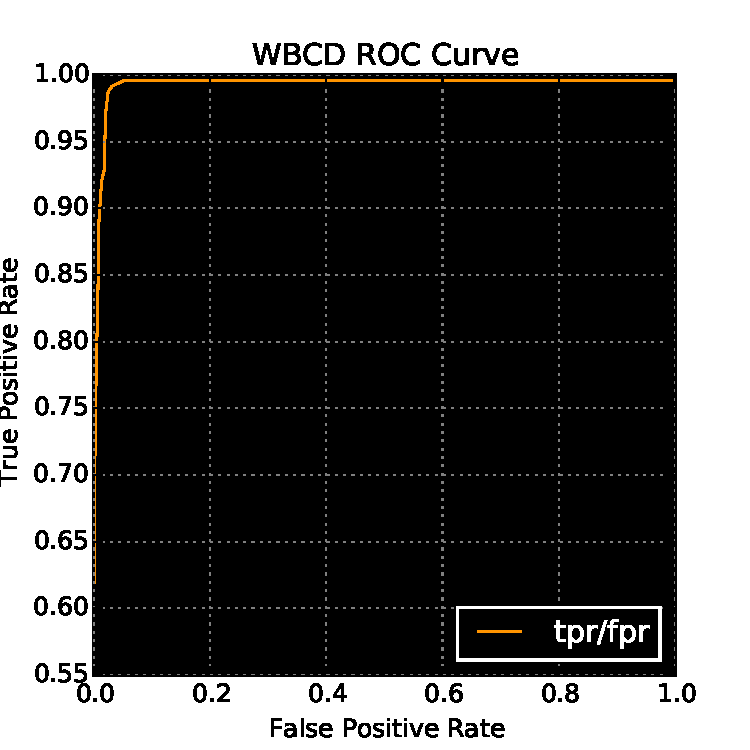
\includegraphics[width=0.95\columnwidth]{figs/wbcd_roc}
\caption {True positive rate as a measure of the false positive rate for a neural network with 14 units at the \nth{1} hidden layer and 13 units at the \nth{2} hidden layer. Network trained for 60 epochs using 10-fold cross validation within each epoch.}
\label{fig:wbcd_roc}

\end{figure}

After deriving the ideal (within our search space) neural network parameters for the WBC data set, we trained a final neural network.
Figure~\ref{fig:wbcd_roc} shows the true positive rate vs. the false positive rate of our model over the WBC data set.
Our model does an extremely good job of predicting true positives without incurring many false positives in the process.
In the context of the WBC data set this is very important because predicting a true positive means catching malignant breast cancer which could lead to treatment and recovery.
The very low false positive rate is important as well because it means that patients will not undergo unnecessary tests and procedures because it was predicted their breast cancer was malignant.

\begin{figure}[t]

\centering
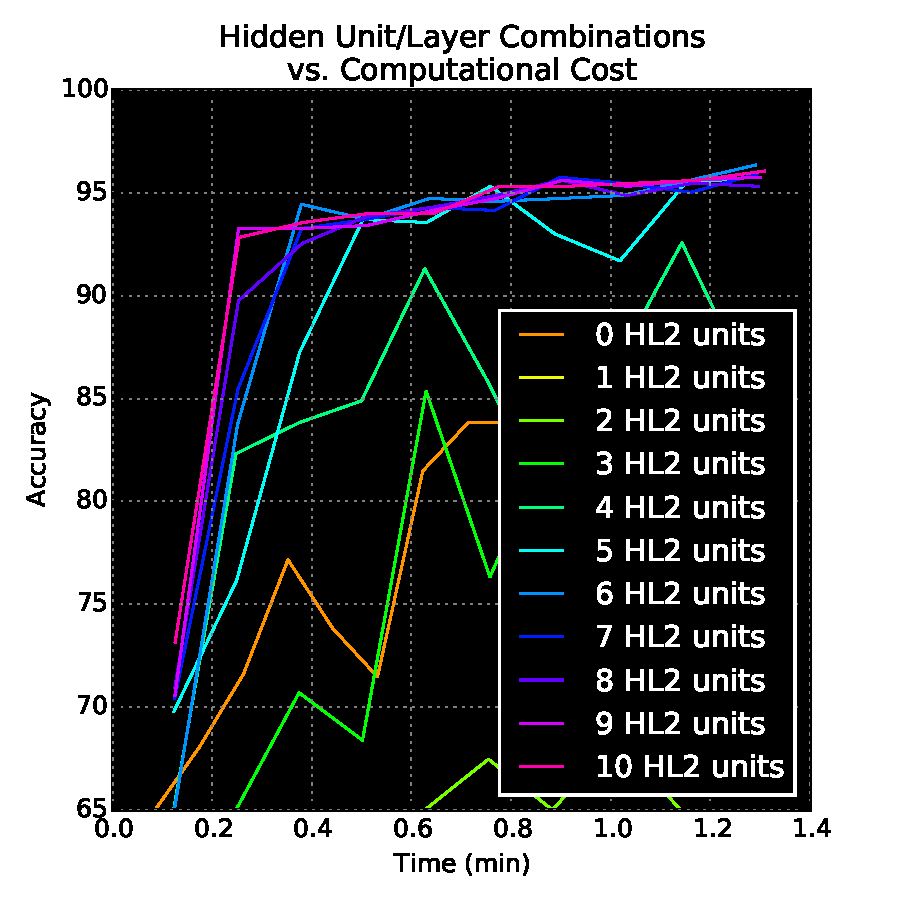
\includegraphics[width=0.95\columnwidth]{figs/wbcd_timing}
\caption {Each line represents the predictive accuracy as a function of computational time required to vary the number of perceptrons in the \nth{1} hidden layer while holding the number of perceptrons in the \nth{2} hidden layer constant ({\em i.e.,} this is equal to generating a row of Figure~\ref{fig:wbcd_table}}
\label{fig:wbcd_timing}

\end{figure}

We have shown the trade offs that can be made with respect to choice of parameters and the predictive accuracy achievable.
However, these trade offs cannot be considered in isolation.
The computational cost of training networks with various parameters needs to be considered as well.
This is because the computational time needed to train a network scales with the number of perceptrons and the number of hidden layers.
When these parameters get sufficiently large the computational time can be on the order of days.

With the WBC data set we don't reach such long run times for training.
Despite this, we are able to demonstrate the effect at a smaller scale.
Figure~\ref{fig:wbcd_timing} shows the computational time required to vary the number of perceptrons in the \nth{1} hidden layer while holding the number of perceptrons in the \nth{2} hidden layer constant.
Each line is the computational effort needed to generate one row from Figure~\ref{fig:wbcd_table}.
Therefore, the time taken to search the entire parameter space from Figure~\ref{fig:wbcd_table} is the sum of these separate lines.
We note that once about 6 perceptrons in the \nth{2} hidden layer are used the accuracy versus time lines stabilize.
If the cost and time of computation were a significant concern then it would be practical to early stop the parameter search space.
However, we do want to point out that Figure~\ref{fig:wbcd_timing} demonstrates that the parameter search can itself be made highly parallel because no line from the figure depends on any other.
Each line is training many separate neural networks.
These computations can proceed in parallel either at the granularity of a line (from Figure~\ref{fig:wbcd_timing}), the granularity of individual networks, or even the granularity of matrix operations within a single network.

\begin{figure}[t]

\centering
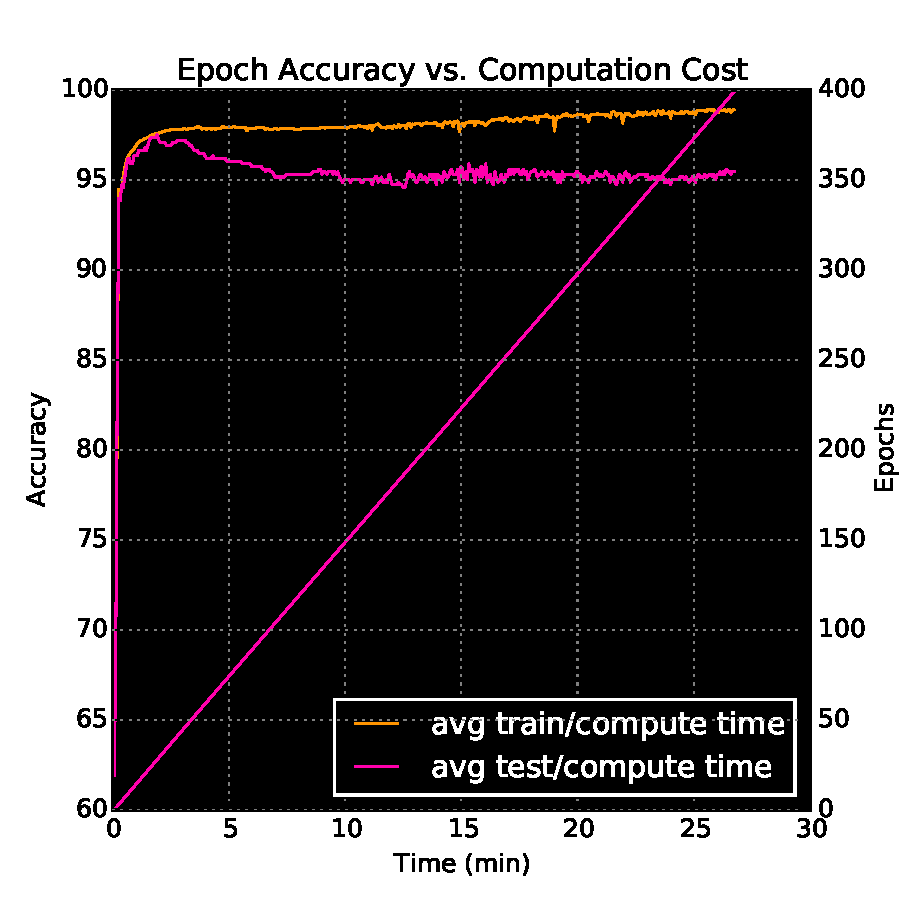
\includegraphics[width=0.95\columnwidth]{figs/wbcd_timing_iterative}
\caption {The predictive accuracy as a function of the computational time required to reach that level of accuracy ({\em i.e.,} the number of epochs trained). The blue line uses the right hand y-axis and indicates the number of epochs \(e\) completed at time \(t\).}
\label{fig:wbcd_iterative_timing}

\end{figure}

In similar style to Figure~\ref{fig:wbcd_timing}, the trade off between the computational cost of training a network for some number of epochs \(e\) versus the predictive accuracy is shown in Figure~\ref{fig:wbcd_iterative_timing}.
It is clear that there is a significant amount of extra computational effort needed to achieve minimal increases in predictive accuracy after about 60 epochs.
Namely, the model has the same predictive accuracy after about 3 minutes of training as it does after about 30 minutes of training.
Even worse, is that the model begins to over fit the data after the 3 minute mark.
Although, overfitting is minimal with the WBC data set, it may be significantly more drastic on a more complicated data set with hundreds of attributes.
As with the previous analysis, there is some parallelism that can be exploited during the epoch parameter space search.

